% To familiarize yourself with this template, the body contains
% some examples of its use.  Look them over.  Then you can
% run LaTeX on this file.  After you have LaTeXed this file then
% you can look over the result either by printing it out with
% dvips or using xdvi.
%

\documentclass[twoside]{article}
%\usepackage{soul}
\usepackage{./lecnotes_macros}


\begin{document}
%FILL IN THE RIGHT INFO.
%\lecture{**LECTURE-NUMBER**}{**DATE**}{**LECTURERS**}{**SCRIBE**}
\lecture{6}{The Retracing Boomerang Attack}{Maria Francis and M. V. Panduranga Rao}{Gautam Singh}{26 March 2025}
%\footnotetext{These notes are partially based on those of Nigel Mansell.}

%All figures are to be placed in a separate folder named ``images''

% **** YOUR NOTES GO HERE:

This is a set of notes for the 2019 retracing boomerang attack paper.

\section{Introduction}

The retracting boomerang attack broke the record for 5-round AES when it was
published, bringing the attack complexity down to \(2^{16.5}\)
encryption/decryption operations. It uncovers a hidden relationship between
boomerang attacks and two other cryptanalysis techniques, namely the yoyo game
and mixture differentials.

\section{Preliminaries}

\subsection{Boomerang Attacks}

The working of a boomerang attack is shown in \autoref{fig:boomerang}. 

\begin{figure}[!ht]
    \centering
    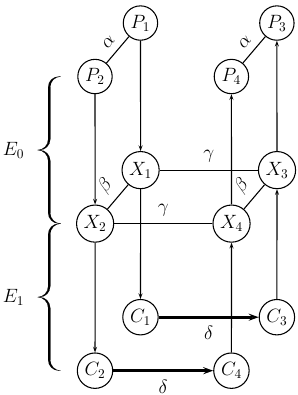
\includegraphics[width=0.25\columnwidth]{images/boomerang.png}
    \caption{The boomerang attack.}
    \label{fig:boomerang}
\end{figure}

Boomerang attacks typically split the encryption function as \(E = E_1 \circ
E_0\), with differential trails for each sub-cipher. Consider \(\alpha
\rightarrow \beta\) to be the differential characteristic in \(E_0\) with
probability \(p\) and \(\gamma \rightarrow \delta\) to be the differential
characteristic in \(E_1\) with probability \(q\). Then, one can build a
distinguisher that can distinguish the full cipher \(E\) from a truly random
permutation in \(\cO\brak{\brak{pq}^{-2}}\) plaintext pairs. This is shown in
\autoref{alg:boomerang-dist}.

\begin{algorithm}
    \caption{The Boomerang Attack Distinguisher}
    \label{alg:boomerang-dist}
    \begin{algorithmic}[1]
        \State Initialize a counter \(ctr \gets 0\). 
        \State Generate \(\brak{pq}^{-2}\) plaintext pairs \(\brak{P_1, P_2}\)
        such that \(P_1 \oplus P_2 = \alpha\).
        \ForAll {pairs \(\brak{P_1, P_2}\)}
            \State Ask for the encryption of \(\brak{P_1, P_2}\) to \(\brak{C_1,
            C_2}\).
            \State Compute \(C_3 = C_1 \oplus \delta\) and \(C_4 = C_2 \oplus 
            \delta\). \Comment{\(\delta\)-shift}
            \State Ask for the decryption of \(\brak{C_3, C_4}\) to \(\brak{P_3,
            P_4}\).
            \If {\(P_3 \oplus P_4 = \alpha\)}
                \State Increment \(ctr\)
            \EndIf
        \EndFor
        \If {\(ctr > 0\)}
            \State \Return This is the cipher \(E\)
        \Else
            \State \Return This is a random permutation
        \EndIf
    \end{algorithmic}
\end{algorithm}

\subsection{The S-box Switch}

\emph{Boomerang switches} aim to gain 1-2 middle-rounds for free by choosing
these differentials carefully. Here, we discuss the S-box switch.

Suppose the last operation in \(E_0\) is a layer of S-boxes applied in parallel,
and this layer \(S\) transforms \(\rho = \brak{\rho_1, \rho_2, \ldots, \rho_t}\)
to \(S\brak{\rho} =
\brak{f_1\brak{\rho_1}\|f_2\brak{\rho_2}\|\ldots\|f_t\brak{\rho_t}}\) for \(t\)
independent keyed functions \(f_i\). Suppose the difference for both \(\beta\)
and \(\gamma\) corresponding to the output of some \(f_j\) is equal to
\(\Delta\). Denoting this part of the intermediate state by \(X_j\), using the
notation of \autoref{fig:boomerang} gives

\begin{equation}
    \brak{X_1}_j \oplus \brak{X_2}_j = \brak{X_1}_j \oplus \brak{X_3}_j = \brak{X_2}_j \oplus \brak{X_4}_j = \Delta
    \label{eq:s-switch}
\end{equation}

which shows \(\brak{X_1}_j = \brak{X_4}_j\) and \(\brak{X_2}_j = \brak{X_3}_j\).
This \emph{S-box switch} shows that if the differential characteristic in
\(f_j^{-1}\) holds for the pair \(\brak{X_1, X_2}\), then it will hold for the
pair \(\brak{X_3, X_4}\). Thus, we pay for probability in one direction, since
the equality is guaranteed to hold in the other direction. In particular, the
overall probability of the distinguisher is increased by a factor of
\(\brak{q^\prime}^{-1}\), where \(q^\prime\) is the probability of the
differential characteristic in \(f_j\).

\subsection{The Yoyo Game}

Like the boomerang attack, the yoyo game starts off by encrypting a pair of
plaintexts \(\brak{P_1, P_2}\) to \(\brak{C_1, C_2}\), then modifying them to
\(\brak{C_3, C_4}\) and decrypting them. However, unlike the boomerang attack,
this process continues in the yoyo game. This process satisfies the property
that \emph{all} pairs of intermediate values \(\brak{X_{2l + 1}, X_{2l + 2}}\)
satisfy some property (such as zero difference in some part). However, the
probability that such a property is satisfied by such a sequence is extermely
low and impractical. Still, the yoyo technique has been used to attack AES
reduced to 5 rounds.

\subsection{Mixture Differentials}

We begin by defining a mixture.

\begin{definition}[Mixture]
    \label{def:mixture}
    Suppose \(P_i \triangleq \brak{\rho_1^i, \rho_2^i, \ldots, \rho_t^i}\).
    Given a plaintext pair \(\brak{P_1, P_2}\), we say \(\brak{P_3, P_4}\) is a
    \emph{mixture counterpart} of \(\brak{P_1, P_2}\) if for each \(1 \le j \le t\),
    the quartet \(\brak{\rho_j^1, \rho_j^2, \rho_j^3, \rho_j^4}\) consists of
    two pairs of equal values or of four equal values. The quartet \(\brak{P_1,
    P_2, P_3, P_4}\) is called a \emph{mixture}.
\end{definition}

From \autoref{def:mixture}, we observe that if \(\brak{P_1, P_2, P_3, P_4}\) is
a mixture, then the XOR of the intermediate values \(\brak{X_1, X_2, X_3, X_4}\)
is zero. Thus, if \(X_1 \oplus X_3 = \gamma\), then \(X_2 \oplus X_4 = \gamma\).
Hence, for a characteristic \(\gamma \xrightarrow{q} \delta\) in \(E_1\), we see
that \(C_1 \oplus C_3 = C_2 \oplus C_4 = \delta\) with probability \(q^2\).

The technique of mixture differentials has been applied to AES reduced up to 6
rounds. Usually \(E_0\) is taken to be the first 1.5 rounds of AES, which can be
treated as four parallel super S-boxes.

\section{The Retracing Boomerang Attack}

The \emph{retracing boomerang} framework contains two attack types - a
\emph{shifting} type and a \emph{mixing} type, both of which are explored below.
Both attacks make use of the setup shown in \autoref{fig:retr-boomerang}.
Although the additional split \(E_1 = E_{12} \circ E_{11}\) looks restrictive,
it applies for a wide class of block ciphers such as SASAS constructions.
Further, we assume that \(E_12\) can be split into two parts of size \(b\) and
\(n - b\) bits, call these functions \(E_{12}^L\) and \(E_{12}^R\), with
characteristic probabilities \(q_2^L\) and \(q_2^R\) respectively.

\begin{figure}[!ht]
    \centering
    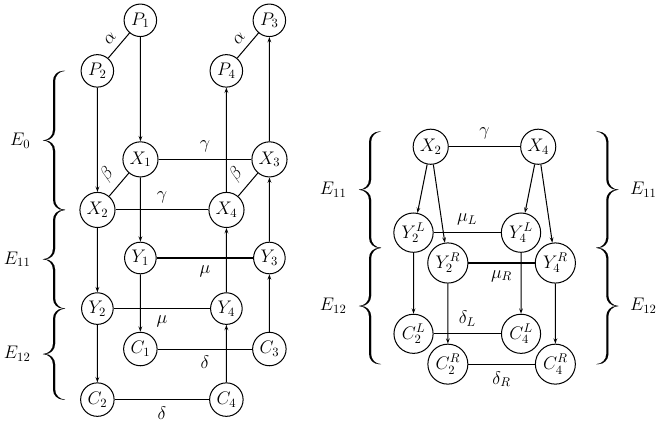
\includegraphics[width=0.5\columnwidth]{images/retracing_boomerang.png}
    \caption{The retracing boomerang attack.}
    \label{fig:retr-boomerang}
\end{figure}

\subsection{The Shifting Retracing Attack}

Assuming that \(pq_1q_2^Lq_2^R \gg 2^{-n/2}\), we can use the standard boomerang
attack to build a distinguisher similar to \autoref{alg:boomerang-dist}. The
main idea of the shifting retracing attack is to add a \(\brak{b - 1}\)-bit
filtering in the middle of the attack procedure, which is to check if \(C_1^L
\oplus C_2^L = 0 \textrm{ or } \delta_L\). We discard all such pairs that do not
satisfy this relation. A \(\delta\)-shift is performed on the filtered
ciphertext pairs to get \(\brak{C_3, C_4}\).

The key idea of performing this filtering is that the two unordered pairs
\(\brak{C_1, C_3}\) and \(\brak{C_2, C_4}\) are \emph{equal}. Thus, if one of
these pairs satisfies the differential characteristic \(\delta_L
\xrightarrow{q_2^L} \mu_L\), the other pair will too, which increases the
probability of the boomerang distinguisher by \(\brak{q_2^L}^{-1}\).

Notice that any possible characteristic of \(\brak{E_{12}^L}\) has probability
at least \(2^{-b + 1}\), thus the overall probability of the distinguisher
increases by a factor of at most \(2^{b - 1}\). On the other hand, the filtering
only leaves \(2^{-b + 1}\) of the pairs, so there is no apparent gain. However,
this approach has the following advantages.

\begin{enumerate}
    \item \emph{Improving the signal to noise ratio.} Improving the probability
    by a factor of \(\brak{q_2^L}^{-1}\) improves the signal to noise ratio
    which ensures a higher fraction of the filtered pairs on average satisfy
    \(P_3 \oplus P_4 = \alpha\). Furthermore, the characteristic \(\beta
    \xrightarrow{p} \alpha\) for the pair \(\brak{X_3, X_4}\) can be replaced by
    a truncated differential characteristic \(\beta \xrightarrow{p^\prime}
    \alpha^\prime\) of higher probability.
    \item \emph{Reducing the data complexity.} Due to the filtering, the attack
    leaves fewer ciphertexts. This improves the complexity in cases where more
    decryption queries are made.
    \item \emph{Reducing the time complexity.} The filtering can also reduce the
    time complexity if it is dominated by the analysis of the plaintext pairs
    \(\brak{P_3, P_4}\).
\end{enumerate}

\subsection{The Mixing Retracing Attack}

In the shifting attack, the attacker forces equality between the unordered pairs
\(\brak{C_1^L, C_2^L}\) and \(\brak{C_3^L, C_4^L}\) using a \(\delta\)-shift.
Instead, in this type of attack, each ciphertext pair can be shifted by
\(\brak{C_1^L \oplus C_2^L, 0}\). The resulting ciphertexts are

\begin{align}
    C_3 &= \brak{C_3^L, C_3^R} = \brak{C_1^L \oplus \brak{C_1^L \oplus C_2^L}, C_1^R} = \brak{C_2^L, C_1^R}, \\
    C_4 &= \brak{C_4^L, C_4^R} = \brak{C_2^L \oplus \brak{C_1^L \oplus C_2^L}, C_2^R} = \brak{C_1^L, C_2^R}.
\end{align}

Again, the unordered pairs \(\brak{C_1^L, C_2^L}\) and \(\brak{C_3^L, C_4^L}\)
are equal. Further, we have \(C_1^R = C_3^R\) and \(C_2^R = C_4^R\), thus we
gain an additional factor of \(\brak{q_2^R}^{-2}\) for a total probability of
\(\brak{pq_1}^2q_2^L\). This mixing is also similar to the core step used in the
yoyo attack on AES.

\subsection{Comparison Between the Two Types of Retracing Attacks}

Although the mixing attack has a higher probability, the shifting attack is
better in various scenarios.

\begin{enumerate}
    \item \emph{Using structures.} In the shifting attack, the same
    \(\delta\)-shift is applied to all pairs of ciphertexts and the filtering is
    applied first to reduce the data complexity. This is not possible in the
    mixing attack since the shift is based on the ciphertext pair and nothing is
    discarded. 
    
    Typically, the basic boomerang attack is extended by adding a round at the
    top or bottom of the distinguisher. In such cases, the shifting attack can
    be used to obtain all ciphertexts, shift all of them by \(\delta\) and then
    decrypt all of them, simulatneously checking for the filter and condition
    between \(P_3\) and \(P_4\) using a hash table.
    
    \item \emph{Combination with \(E_{11}\).} In the mixing variant, the output
    difference of \(E_{12}^L\) is arbitrary and changes with each ciphertext
    pair. In most cases, there is no good combination between differential
    characteristics of \(\brak{E_{12}^L}^{-1}\) and \(\brak{E_{11}}^{-1}\) that
    can be used. For instance, in the yoyo attack, \(E_{11}\) is empty.

    \item \emph{Construction of `friend pairs'.} `Friend pairs' are pairs that
    are attached to other pairs which satisfy a common property. There are many
    more `friend pairs' that can be constructed in the shifting variant, making
    it advantageous.
\end{enumerate}

\section{Retracing Boomerang Attack on 5-round AES}

The retracing boomerang attack is based on the yoyo attack, which is described
first.

\subsection{The Yoyo Attack on 5-round AES}

The yoyo attack decomposes 5-round AES as \(E = E_{12} \circ E_{11} \circ E_0\)
where \(E_0\) consists of the first 2.5 rounds, \(E_{11}\) is the first MC
operation of round 2 and \(E_{12}\) consists of rounds 3 and 4. 

For \(E_0\) in the forward direction, the adversary uses a trucated differential
characteristic whose input difference is zero in three inverse shifted columns
and whose output difference is zero in a single shifted column. Specifically,
\(P_1 = \brak{0, i, 0, 0}\) and \(P_2 = \brak{z, z \oplus i, 0, 0}\) for some
random nonzero \(z\) \emph{after} the SR operation of round 0 has been applied.
The probability of this characteristic is \(4 \cdot 2^{-8} = 2^{-6}\), since it
holds iff the output difference of the active column in round 0 is zero in at
least one byte.

For \(E_{12}\) in the backward direction, notice that 1.5 rounds of AES can be
taken as 4 32-bit super S-boxes. For each ciphertext pair \(\brak{C_1, C_2}\),
the adversary modifies it into its mixture \(\brak{C_3, C_4}\) with respect to
the super S-boxes and asks for their decryption. Due to the mixture
construction, the four inputs to the S-boxes have an XOR of zero, therefore
\(X_1 \oplus X_2 \oplus X_3 \oplus X_4 = 0\) as well since MC is linear.
Therefore, with probability \(2^{-6}\), we have \(X_3 \oplus X_4 = 0\) in a
shifted column. Subsequently, \(Z_3 \oplus Z_4 = 0\) in an inverse shifted
column, which corresponds to one of the four quartets \(\brak{0,5,10,15},
\brak{1,4,11,14}, \brak{2,5,8,13}, \brak{3,6,9,12}\). This can be used to set up
an attack on bytes \(\brak{0,5,10,15}\) of the subkey \(k_{-1}\). To get more
information about \(k_{-1}\), friend pairs of \(\brak{Z_3, Z_4}\) are used.

The yoyo attack has data complexity about \(2^9\) and overall time complexity
\(2^{40}\).

\end{document}
